\documentclass[border=2mm]{standalone}
\usepackage{pgfplots}
\usepackage{amsmath}
\usepackage[scaled]{helvet}
\usepackage[T1]{fontenc}
\renewcommand\familydefault{\sfdefault}
\usepackage[eulergreek]{sansmath}
\pgfplotsset{
tick label style = {font=\sansmath\sffamily}}

\pgfkeys{/pgf/number format/fixed, /pgf/number format/precision=5, /pgf/number format/.cd, 1000 sep = {}}
\pgfplotsset{compat=newest}

\begin{document}

\pgfmathdeclarefunction{gauss}{2}{\pgfmathparse{1/(#2*sqrt(2*pi))*exp(-((x-#1)^2)/(2*#2^2))}%
}

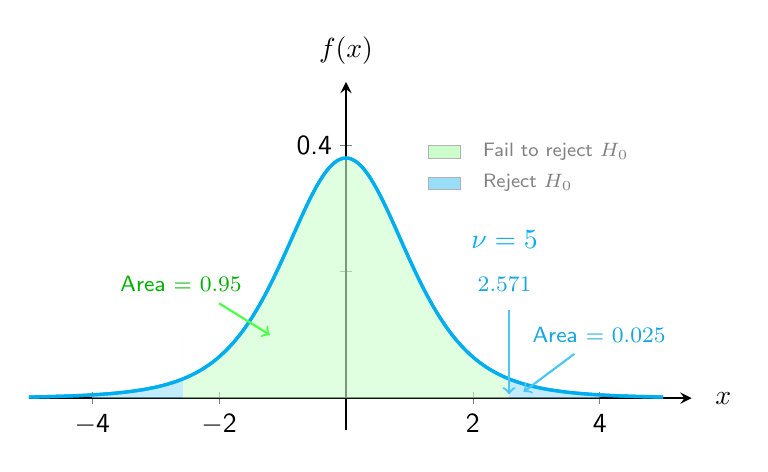
\begin{tikzpicture}[
    declare function={gamma(\z)=
    2.506628274631*sqrt(1/\z)+ 0.20888568*(1/\z)^(1.5)+ 0.00870357*(1/\z)^(2.5)- (174.2106599*(1/\z)^(3.5))/25920- (715.6423511*(1/\z)^(4.5))/1244160)*exp((-ln(1/\z)-1)*\z;},
    declare function={student(\x,\n)= gamma((\n+1)/2.)/(sqrt(\n*pi) *gamma(\n/2.)) *((1+(\x*\x)/\n)^(-(\n+1)/2.));}
]
\begin{axis}[
    width=10cm, % Set the width of the axis
    height=6cm, % Set the height of the axis
    scaled ticks=false,
    axis lines=center,
    enlargelimits=upper,
    line width=0.8,
    xlabel = {$x$},
    ylabel = {$f(x)$}, 
    yticklabel = \empty,
    xmin = -5, xmax = 4.5,
    ymin = -0.05, ymax = 0.45,
    every axis x label/.style={at={(ticklabel* cs:1.02)}, anchor=west,}, every axis y label/.style={at={(ticklabel* cs:1.02)}, anchor=south}
]
% \addplot + [smooth, mark=none, domain=-4:4, samples=100, color=red, line width=1.5] {gauss(0,1)};

% \pgfplotsinvokeforeach{1}{
%     \addplot [thick, smooth, domain=-5:5, samples=100, color=blue, line width=1.2] {student(x,#1)};
% }
% \node at (2.5,0.2) {\color{blue}$\nu=1$};
\pgfplotsinvokeforeach{5}{
    \addplot [thick, smooth, domain=-5:5, samples=100, color=cyan, line width=1.2] {student(x,#1)};
}
% \node at (2.5,0.25) {\color{cyan}$\nu=5$};

% \node at (-0.5,0.4) {\scriptsize$0.4$};

\begin{scope}
    \clip (2.571,0) rectangle (4,0.45);
    \fill[cyan!40, opacity=0.6] plot[domain=2.571:5, samples=100, smooth] (\x,{student(\x,5)}) -- (5, 0) -- (2.571, 0) -- cycle;
\end{scope}

\begin{scope}
    \clip (-2.571,0) rectangle (-4,0.45);
    \fill[cyan!40, opacity=0.6] plot[domain=-5:-2.571, samples=100, smooth] (\x,{student(\x,5)}) -- (-2.571, 0) -- (-5, 0) -- cycle;
\end{scope}

    \begin{scope}
        \clip (-2.571,0) rectangle (2.571,0.4);
        \fill[green!20, opacity=0.6] plot[domain=-2.571:2.571, smooth] (\x,{student(\x,5)}) -- (2.571, 0.1) -- (2.571, 0) -- (-2.571, 0) -- (-2.571, 0.1) -- cycle;
    \end{scope}

\draw[draw=gray!60, line width=0.1, fill=green!20] (1.3,0.38) rectangle (1.8,0.40);
\draw[right] (2,0.39) node {\scriptsize\color{gray}Fail to reject $H_0$};
\draw[draw=gray!60, line width=0.1, fill=cyan!40] (1.3,0.32+0.01) rectangle (1.8,0.34+0.01);
\draw[right] (2,0.33+0.01) node {\scriptsize\color{gray}Reject $H_0$};

% \addplot [thick, smooth, domain=-5:5, samples=100, color=cyan, line width=1.2] {student(x,1)};

\pgfplotsinvokeforeach{5}{
    \addplot [thick, smooth, domain=-5:5, samples=100, color=cyan, line width=1.2] {student(x,#1)};
}
\node at (2.5,0.25) {\color{cyan}$\nu=5$};

\node at (-0.5,0.4) {0.4};

\draw[arrows=<-, thick, color=cyan!70] (2.571,0.006)--(2.571,0.14);
\node at (2.5,0.18) {\footnotesize\color{cyan!90!black}$2.571$};

% \draw[arrows=<-, thick, color=red!70] (0.816,0.002)--(0.816,0.06);
% \node at (0.816,0.10) {\footnotesize\color{red!90!black}$t\approx 0.816$};

\draw[arrows=<-, thick, color=cyan!70] (2.8,0.01)--(3.6,0.07);
\node at (3.99,0.1) {\footnotesize\color{cyan!90!black}Area = $0.025$};

\draw[arrows=<-, thick, color=green!70] (-1.2,0.1)--(-2,0.15);
\node at (-2.6,0.18) {\footnotesize\color{green!70!black}Area = $0.95$};

\end{axis}
\end{tikzpicture}

\end{document}